\speaker{\Mathieu}
\subsection{} % PAs besoin de titre



\begin{frame}
\frametitle{UNICEF 76}
\framesubtitle{Cahier des charges}
	\begin{itemize}
		\item Plaidoyers dans les \'ecoles
		\item Actions frimousses
		\item Villes Amies des Enfants
		\item Ventes ponctuelles
	\end{itemize}
	
	Mettre autre chose
\end{frame}




\begin{frame}
	\frametitle{swag}
	\framesubtitle{Maxi swag}
	\begin{figure}
		\centering
		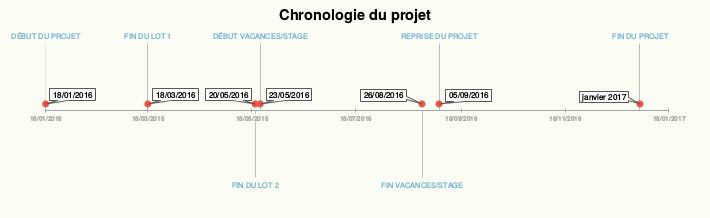
\includegraphics[scale=0.65]{images/planningProjet1.jpeg}
	\end{figure}
	Est ce qu'on met un tire ? je pense que oui mais bon 
\end{frame}




\begin{frame}
	\frametitle{Lot 1}
	Architecture matérielle et logicielle du projet
\end{frame}


\speaker{\Michel}
\begin{frame}
	\frametitle{Lot 2}
	Couvre la partie plaidoyer :
	\begin{itemize}
		\item Gestion des utilisateurs
		\item Gestion des établissements
		\item Gestion de l'envoie des différents emails
	\end{itemize}
\end{frame}

\begin{frame}
	\frametitle{Lot 3}
	Couvre la partie frimousses :
	\begin{itemize}
		\item Envoie d'un formulaire aux établissements
		\item Affecter un bénévole en charge du dossier
	\end{itemize}
\end{frame}


\begin{frame}
	\frametitle{Lot 4}
	Couvre la partie actions ponctuelles
	\begin{itemize}
		\item Géolocalisation des stands
		\item Affectation des créneaux aux bénévoles
		\item Email de rappel
		\item Gestion des chiffres d'affaires
		\item Gestion des stocks
	\end{itemize}
\end{frame}